\documentclass[12pt]{article}
\usepackage{graphicx}
\usepackage{lscape}
\usepackage{listings}
\usepackage[demo]{graphicx}
\usepackage{subfig}
\usepackage{hyperref}

\usepackage[dvipsnames]{xcolor}
\colorlet{LightRubineRed}{RubineRed!70}
\colorlet{Mycolor1}{green!10!orange}
\definecolor{Mycolor2}{HTML}{00F9DE}
%
\pagecolor{black}
\color{white}
%
% Title[Enter title of the experiment here]
\title{EE230: Analog Circuits Lab\\Square Root Amplifier\\Lab No. 4}
% Author[Enter details of author here]
\author{Anupam Rawat, 22b3982}
\date{Janurary 25, 2024}
% begin the document.
\begin{document}

% make a title page.[this creates title page]
\maketitle

\section{Aim of the experiment}
Construct a square root amplifier and fine tune it to utmost precision

\section{Design}

The current through the diode in forward bias is given by the following equation
 \begin{equation}
     I_D = I_S * (e^{V_D}^/^{n V_T} - 1)
 \end{equation}     
Rearranging the terms we get
\begin{equation}
    V_D = n\cdot V_T * (ln(I_D) - ln(I_S))
\end{equation}
The output of Block-1 is given by $V_{out1}$:
\begin{equation}
    V_{out1} = - V_D = n\cdot V_T * (ln(I_S R) - ln(V_{in}))
\end{equation}
The output of Block-2 is given by $V_{out2}$:
\begin{equation}
    V_{out2} = - n\cdot V_T\cdot ln(I_S R) + (ln(V_{in})) V_T \cdot n + 2 V_{b1}
\end{equation}
We can remove the offset terms which don't include $V_{in}$ by choosing: 
\begin{equation}
    V_{b1} = \frac{n \cdot V_T \cdot ln(I_S\cdot R)}{2}
\end{equation}
\begin{equation}
    V_{out2} = n\cdot V_T\cdot ln(V_{in})
\end{equation}
The output of Block-3 can be given by:
\begin{equation}
    V_{out3} = - \frac{R_{22}}{R_{21}} \cdot V_{out2} = - \frac{R_{22}}{R_{21}} \cdot V_T\cdot ln(V_{in}) = ln(V_{in} ^- ^\frac{R_{22}}{R_{21}} ^n ^VT)
\end{equation}
For Block-4, $V_x$ = $V_{b2}$ (virtual ground) and:
\begin{equation}
     \hypertarget{equation(8)}{ V_{out} = R_3\cdot I_{D2} + V_{b2} = R_3\cdot T_{S2}\cdot e^\frac{V_{b2}}{n_2\cdot V_T} {V_{in}}^\frac{n_1}{n_2}^\frac{R_{22}}{R_{21}} + V_{b2} }
\end{equation}
We can simplify the circuit as:
\begin{equation}
    \hypertarget{equation(9)}{V_{R3} = V_{out} - V_x = \beta_1 \cdot V_{in}^\beta^2}
\end{equation}
For square root amplifier, we can choose $\beta_1$ = 1 and $\beta_2$ = $\frac{1}{2}$

 \begin{figure}[h!]
\centering
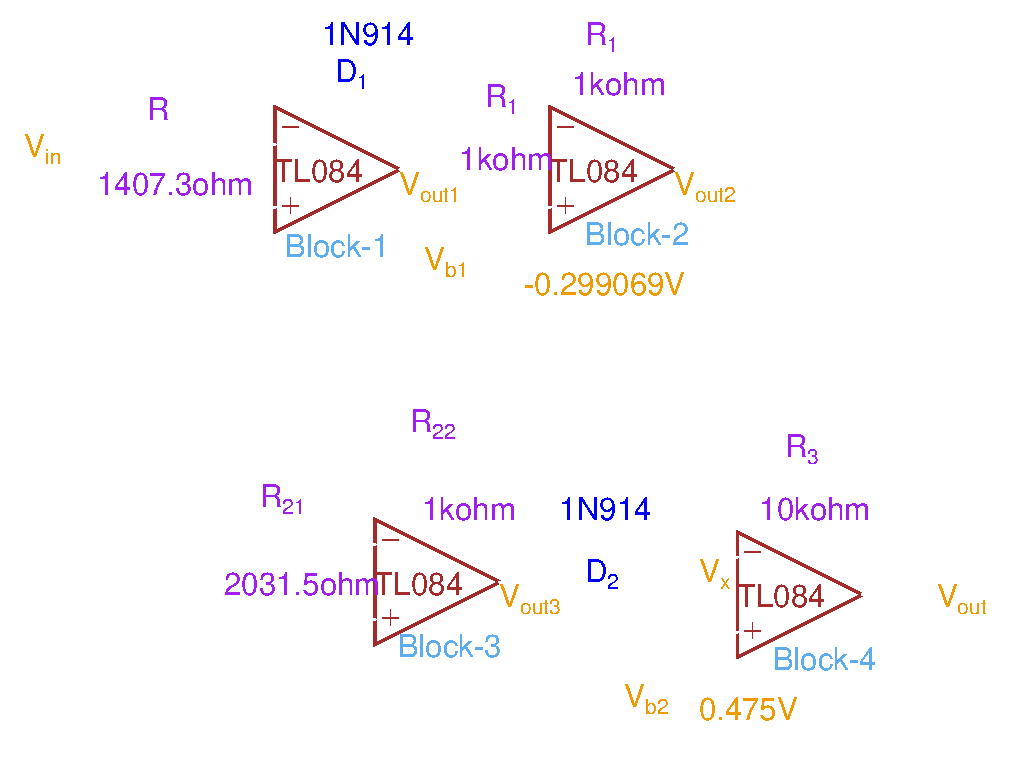
\includegraphics[scale = 0.8]{Modified_Circuit_Design.eps}
\caption{Circuit Diagram}
\end{figure}
\newpage

\begin{landscape}
    \section{Simulation Results}
    
    \begin{figure}[h!]
        \centering
        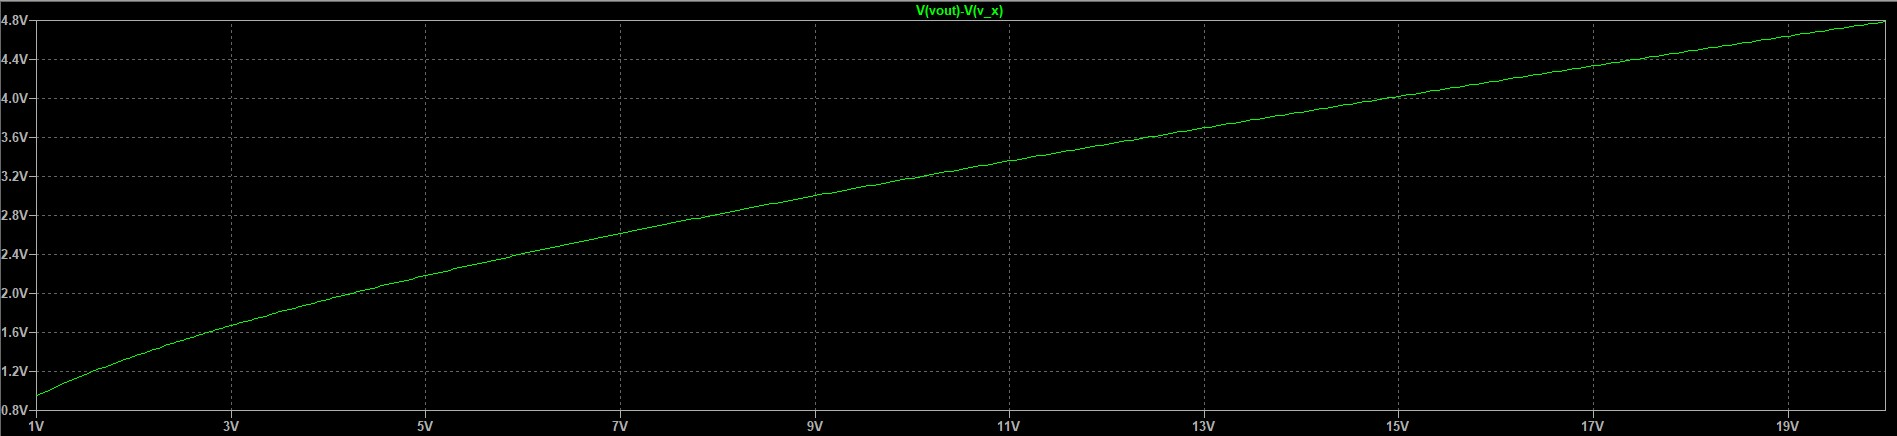
\includegraphics[scale = 0.45]{Sim_4_1.jpg}
    \end{figure}

    \begin{figure}[h!]
        \centering
        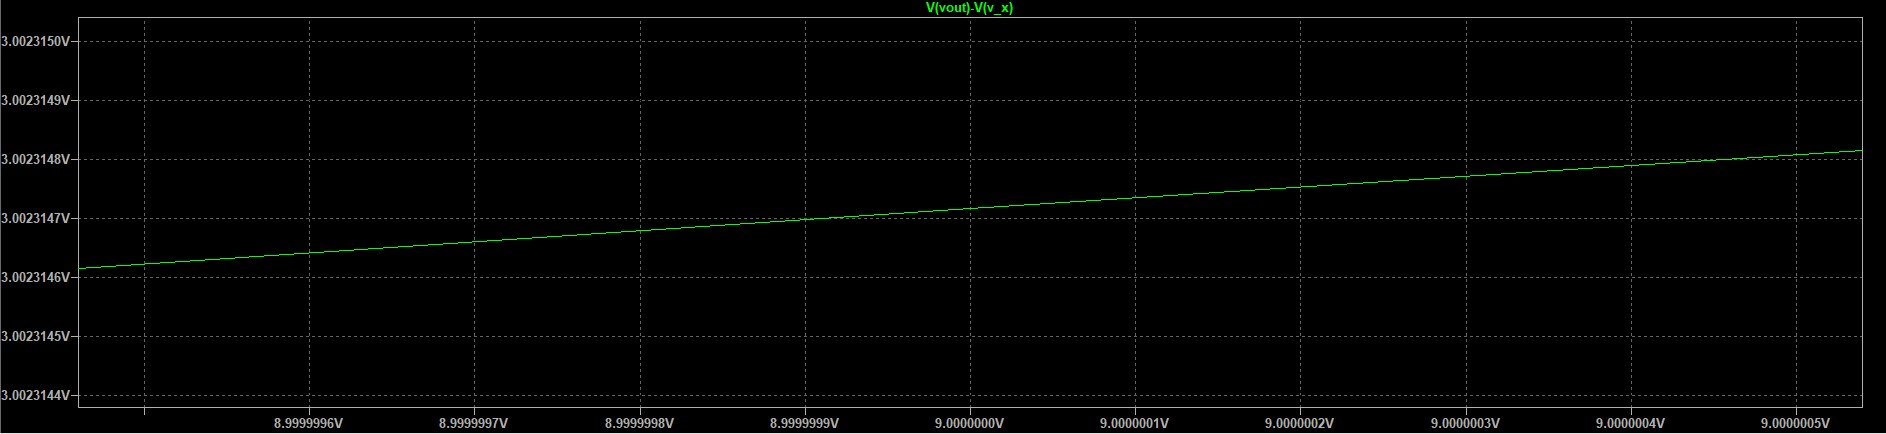
\includegraphics[scale = 0.455]{Sim_4_2.jpg}
    \end{figure}
\end{landscape}

\newpage

\section{Circuit Schematics}
    \begin{figure}[h!]
        \hspace{-38mm}
        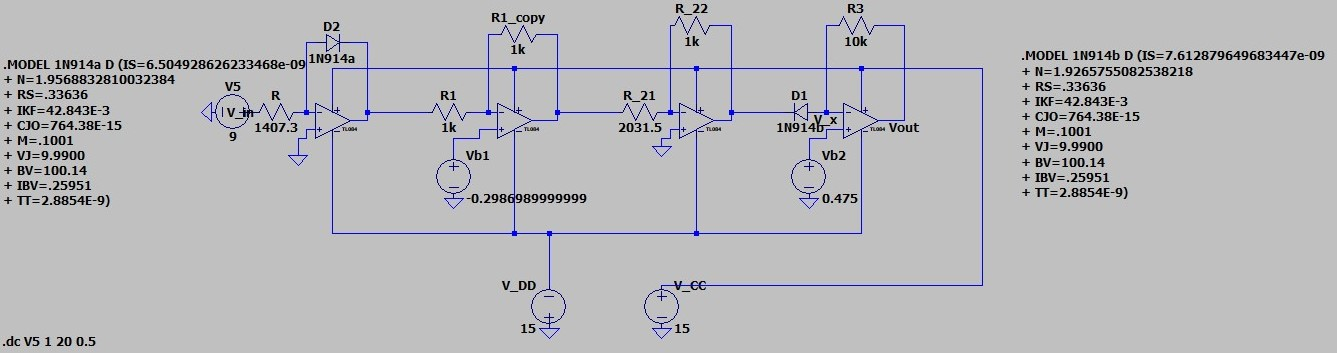
\includegraphics[scale = 0.6]{Sim_4_3.jpg}
    \end{figure}

\section{Experimental results}
\subsubsection*{\textit{\underline{Plot $ln(I_D)$ v/s $V_D$}}:}
\hspace{-5cm}
\begin{figure}[h!]
    \subfloat[\centering]{{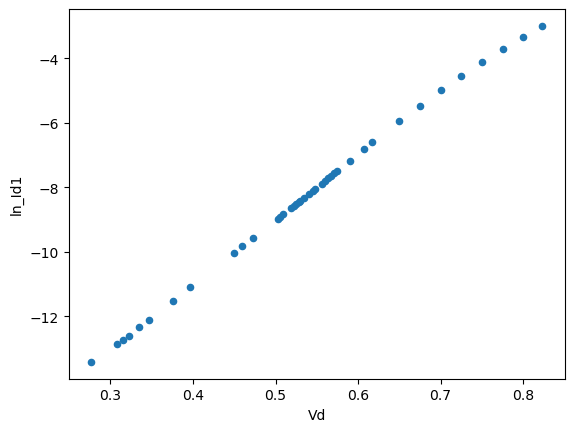
\includegraphics[width=8cm]{wo_linregress_ln(I_D1)_vs_V_d.png} }}%
    \qquad
    \subfloat[\centering]{{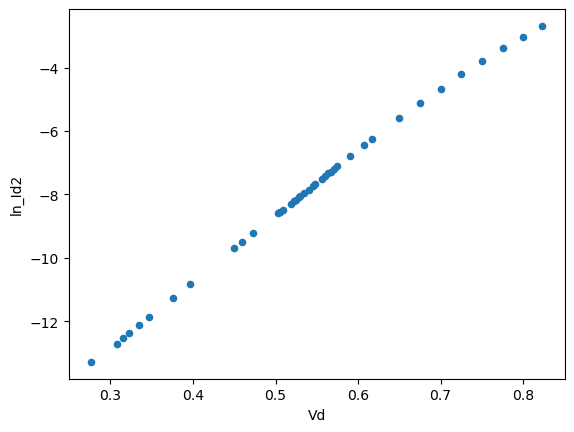
\includegraphics[width=8cm]{wo_linregress_ln(I_D2)_vs_V_d.png} }}%
\end{figure}

\begin{figure}[h!]
    \subfloat[\centering]{{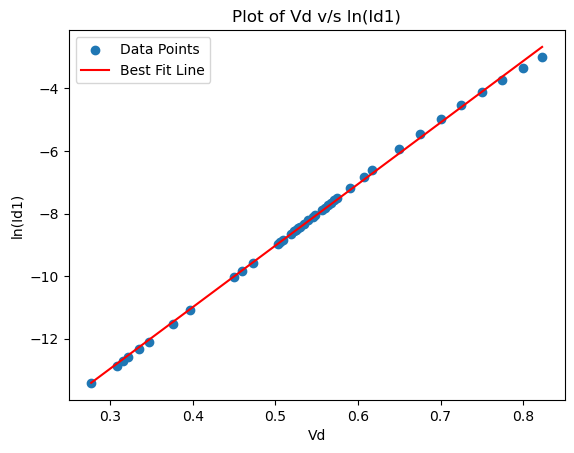
\includegraphics[width=8cm]{ln(I_D1)_vs_V_d.png} }}%
    \qquad
    \subfloat[\centering]{{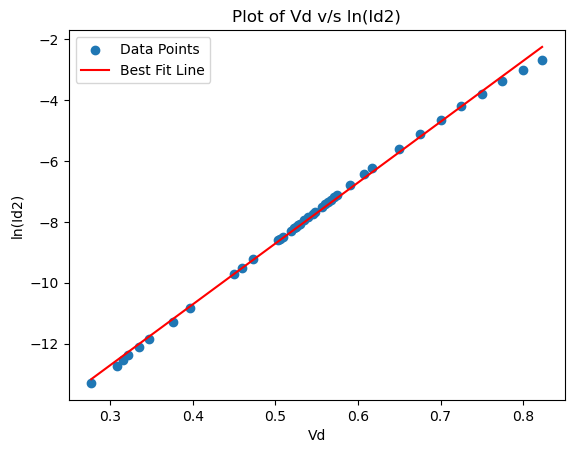
\includegraphics[width=8cm]{ln(I_D2)_vs_V_d.png} }}%
\end{figure}

\begin{figure}[h!]
    \centering
    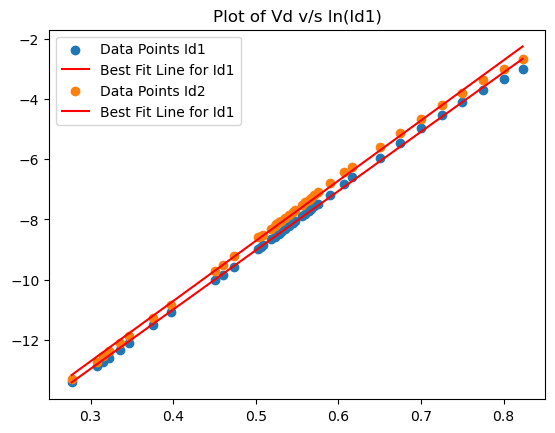
\includegraphics[scale=0.8]{combined_plot.png}
\end{figure}

\subsubsection*{\textit{\underline{manually identify the range over which ln($I_D$) is a linear function of $V_D$}}:}
As it can be seen from the figure (a) on the top of this page, the last point to be on the line is, the values of which are - $V_D$ = 0.75, $I_{D1}$ = 0.01633 and $V_D$ = 0.725 and $I_{D2}$ = 1.48e-02

\subsubsection*{\textit{\underline{determine $I_S$ and n}}:}
The value of: \\
$I_{S1}$ = $\frac{1}{e^18.8507}$ = 6.5e - 9 \hspace{2cm} $n_1$ = $\frac{1}{slope_1\cdot V_T}$ = $\frac{1}{19.65\cdot 0.026}$ = 1.95 \\
$I_{S2}$ = $\frac{1}{e^18.6934}$ = 7.6e - 9 \hspace{2cm} $n_2$ = $\frac{1}{slope_2\cdot V_T}$ = $\frac{1}{19.96\cdot 0.026}$ = 1.926 \\

\subsubsection*{\textit{\underline{Choose diode for Block-1 and determine the value of R}}:}
We'll choose Diode 1 since it's correlation is more i.e. it's linear over a larger range as compared to Diode 2.
$I_{D1}$ = 0.01066, R = $\frac{15}{I_{D1}}$ = $\frac{15}{0.01066}$ = 1407.13$\Omega$

\subsubsection*{\textit{\underline{Determine the expression for $V_{out1}$}}:}
$V_{out1}$ = n  $V_T$  (ln($I_S$ R) - ln($V_{in}$)) = 0.0508(-11.6 - ln($V_{in}$))

\subsubsection*{\textit{\underline{Determine $V_{b1}$ to remove offset and choose $R_1$ arbitrarily}}:}
$V_{b1}$ = $\frac{n V_T ln(I_S R)}{2}$ = -0.0294 V and choosing $R_1$ = 1k$\Omega$. Corresponding $V_{out1}$ becomes -0.589V.

\subsubsection*{\textit{\underline{Select $V_{b2}$ and $R_3$ such that $V_{R3}$ = 1V}}:}
choosing $R_3$ = 10k$\Omega$\\
and substituting the values in \hyperlink{equation(8)}{equation (8)} and \hyperlink{equation(9)}{equation (9)}, we get, $V_{R3}$ = 0.475 for $R_3$ = 10k$\Omega$, $I_{S2}$ = 7.6e-09, $n_2$ = 19.96 and $V_T$ = 0.026.

\subsubsection*{\textit{\underline{Choose $R_{21}$ and $R_{22}$ and also fine tune for finding sqrt when $V_{in}$=9V}}:}
We want \hyperlink{equation(9)}{$\beta_2$ = $\frac{1}{2}$} OR $\frac{n_1}{n_2}\cdot\frac{R_{22}}{R_{21}}$ = $\frac{1}{2}$\\ $R_{21}$ = 2.03 * $R_{22}$. Let's take $R_{22}$ = 1k$\Omega$, $R_{21}$ = 2.03k$\Omega$. \\
When we fine tune the circuit, we get, $V_{b1}$ = -0.2980989999999V.
\section{Experiment completion status}
The full experiment along with the handwritten reports was completed during the lab hours.
\end{document}
